\documentclass[a4paper,10pt,oneside,openany]{book}
\usepackage[utf8]{inputenc}
\usepackage{amsmath}
\usepackage{cancel}
\usepackage{amsfonts}
\usepackage{amssymb}
\usepackage{xcolor}
\usepackage{mathrsfs}
\usepackage{amsfonts}
\usepackage{amsmath}
\usepackage{mathtools}
\usepackage{centernot}
\usepackage{graphicx}
\usepackage{setspace}
\usepackage{geometry}
\usepackage{tcolorbox}
\usepackage{hyperref}
\usepackage{stackengine}
\usepackage{bm} %bold math
%%%%%%%%%%%%%%%%%%%%%%%%%%%%%%%%%%%%%%%%%%%%%%%%%%%%%%%%%%%%%%%%%%%%%%%%%%%%%%%%%%%%%%%%%%%%%%%%%%
\usepackage{multicol}

%%%%%%%%%%%%%%%%%%%%%%%%%%%%%%%%%%%%%%%%%%%%%%%%%%%%%%%%%%%%%%%%%%%%%%%%%%%%%%%%%%%%%%%%%%%%%%%%%%
\usepackage{listings}
\usepackage{color}
\usepackage{qtree}

\definecolor{dkgreen}{rgb}{0,0.6,0}
\definecolor{gray}{rgb}{0.5,0.5,0.5}
\definecolor{mauve}{rgb}{0.58,0,0.82}

\lstset{frame=tb,
  language=C++,
  aboveskip=3mm,
  belowskip=3mm,
  showstringspaces=false,
  columns=flexible,
  basicstyle={\small\ttfamily},
 %numbers=left,
  numbers=none,
  numberstyle=\tiny\color{gray},
  keywordstyle=\color{blue},
  commentstyle=\color{dkgreen},
  stringstyle=\color{mauve},
  breaklines=true,
  breakatwhitespace=true,
  tabsize=3,
  %xleftmargin=0.5cm
}
%%%%%%%%%%%%%%%%%%%%%%%%%%%%%%%%%%%%%%%%%%%%%%%%%%%%%%%%%%
\usepackage{graphicx}
\graphicspath{ {images/} }

\definecolor{grigio}{RGB}{179,179,179}
%\theoremstyle{plain}
\newtheorem{thm}{Teorema}[section]
\newtheorem{deff}{Definizione}[section]
\newtheorem{dimm}{Dimostrazione}[section]

\geometry{a4paper,top=1.5cm,bottom=1.5cm,left=2.5cm,right=2.5cm,%
heightrounded,bindingoffset=5mm}

\newcommand{\tb}[1]{\textbf{#1}}
\newcommand{\e}[1]{\textit{#1}}
\newcommand{\DEF}[1]{\textcolor{blue}{DEF:}}
\newcommand{\om}[0]{$\Omega$}
\newcommand{\al}[0]{$\mathcal{A}$}
\newcommand{\zero}[0]{$\emptyset$}
\newcommand{\ap}[0]{$\in$}
\newcommand{\im}[0]{$\implies$}

\setcounter{tocdepth}{1} %il grado di profondita indice, 1 solo chapter, 2 section ...

\title{LFC (Soluzione Appello Gennaio 2018)}
\begin{document}
\maketitle
\tableofcontents
\chapter{Esercizio 1}

\subsection{Testo}

\begin{center}
    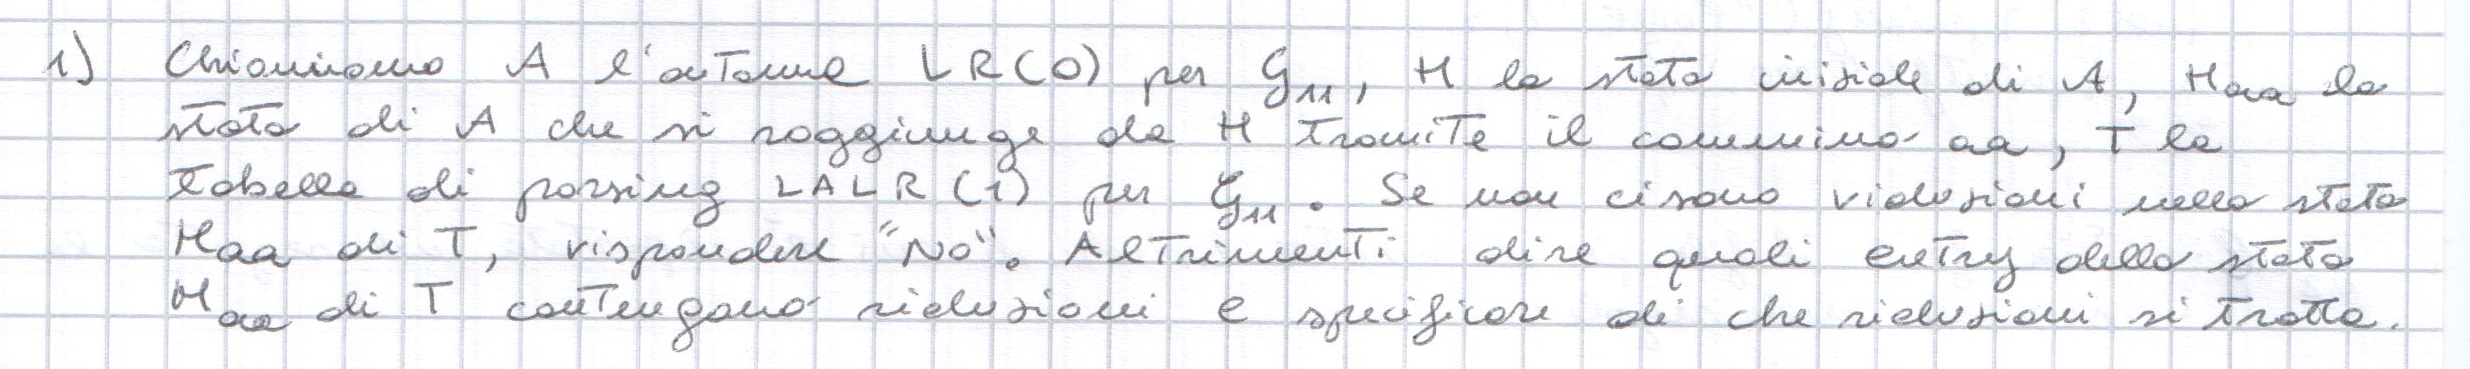
\includegraphics[scale=0.2]{Chapters/Img/01text.png}\\
\end{center} 

\subsection{Soluzione}

\begin{center}
    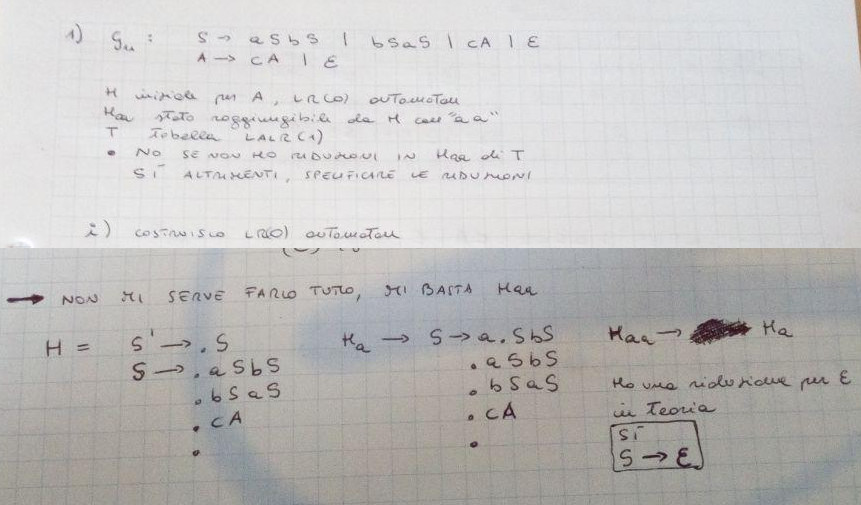
\includegraphics[scale=0.6]{Chapters/Img/01solution.png}\\
\end{center} 

\subsection{Risposta}
S\'i: $S \rightarrow \varepsilon$
\chapter{Esercizio 2}

\subsection{Testo}

\begin{center}
    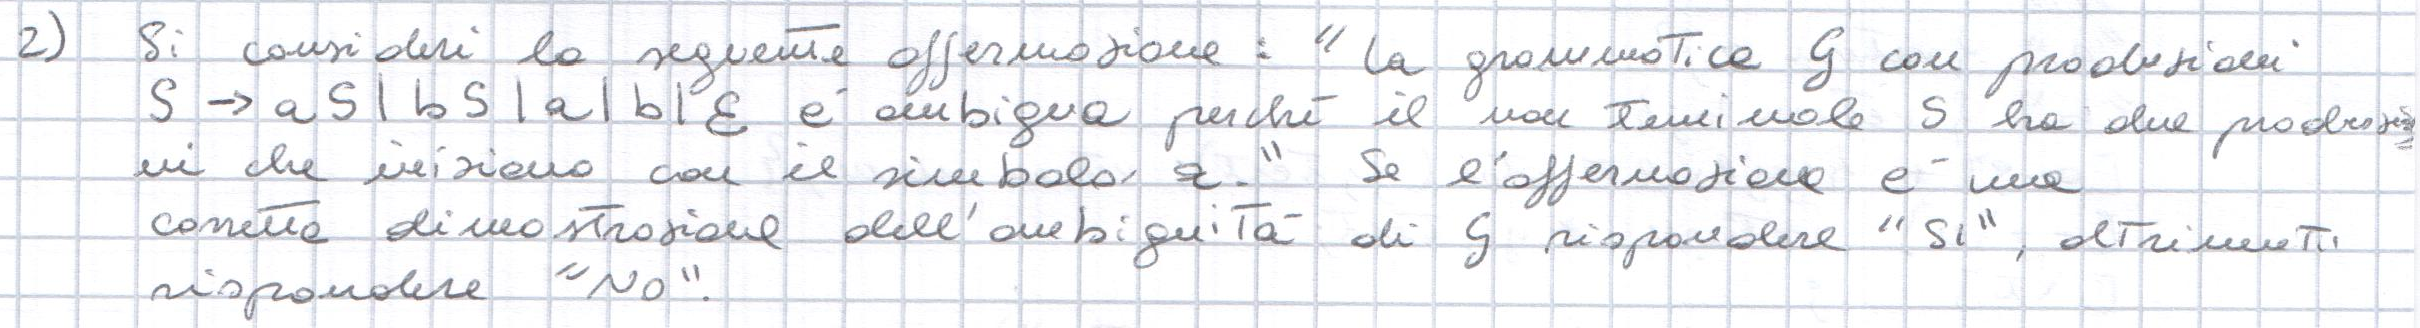
\includegraphics[scale=0.2]{Chapters/Img/02text.png}\\
\end{center} 

\subsection{Soluzione}
\'E vero che la grammatica \'e ambigua ma non perch\'e ci sono le \lq\lq a\rq\rq ma perch\'e \'e fattorizzabile.

\subsection{Risposta}
No
\chapter{Esercizio 3}

\subsection{Testo}

\begin{center}
    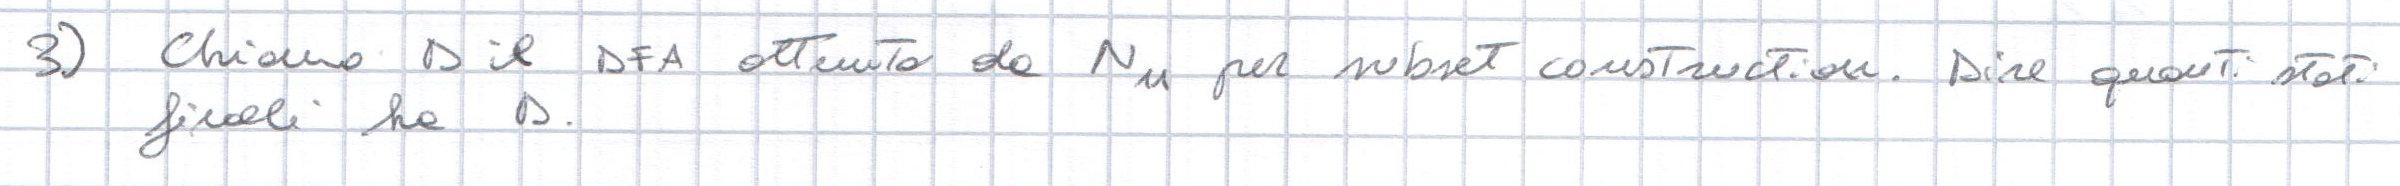
\includegraphics[scale=0.2]{Chapters/Img/03text.png}\\
\end{center} 

\subsection{Soluzione}

\begin{center}
    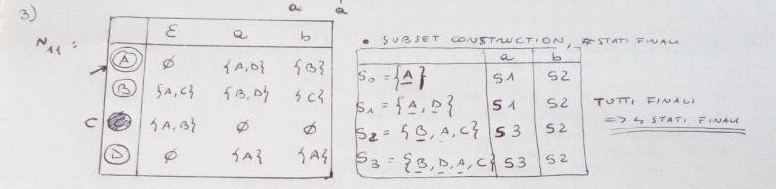
\includegraphics[scale=0.6]{Chapters/Img/03solution.png}\\
\end{center} 

\subsection{Risposta}
4 stati finali dato che A \'e finale e tutti gli insiemi contengono A.
\chapter{Esercizio 4}

\subsection{Testo}

\begin{center}
    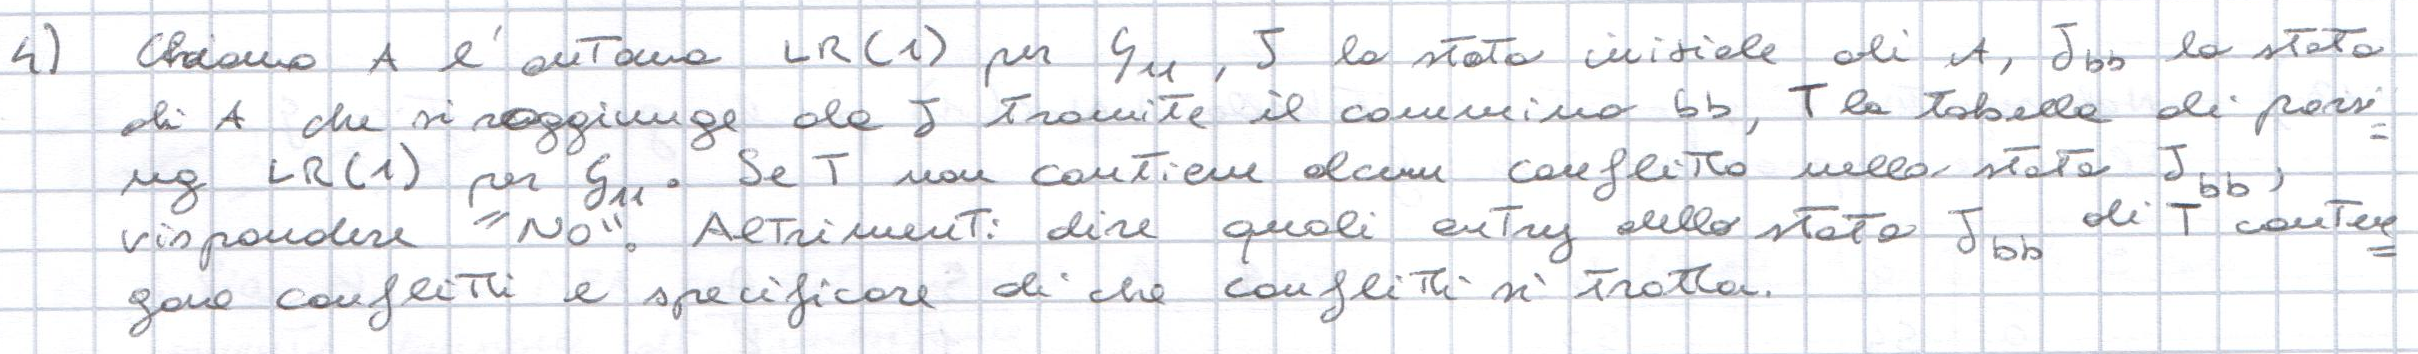
\includegraphics[scale=0.2]{Chapters/Img/04text.png}\\
\end{center} 

\subsection{Soluzione}

\begin{center}
    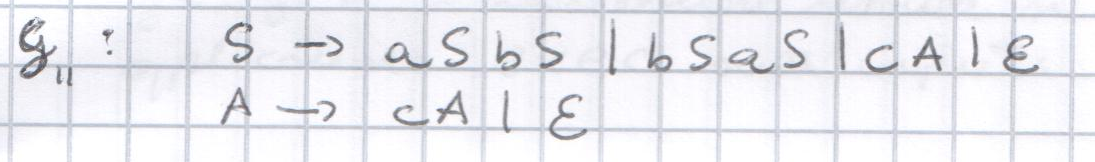
\includegraphics[scale=0.4]{Chapters/Img/g11.png}
    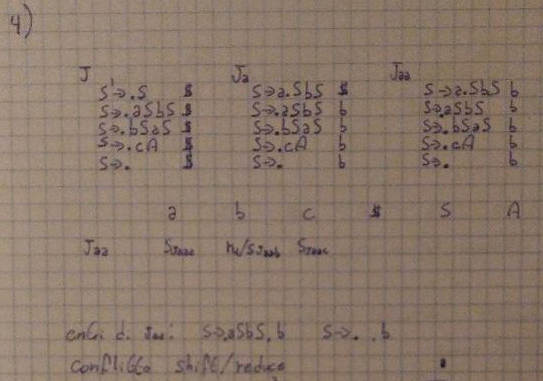
\includegraphics[scale=0.6]{Chapters/Img/04solution.png}\\
\end{center} 

%\subsection{Risposta}

\chapter{Esercizio 5}

\subsection{Testo}

\begin{center}
    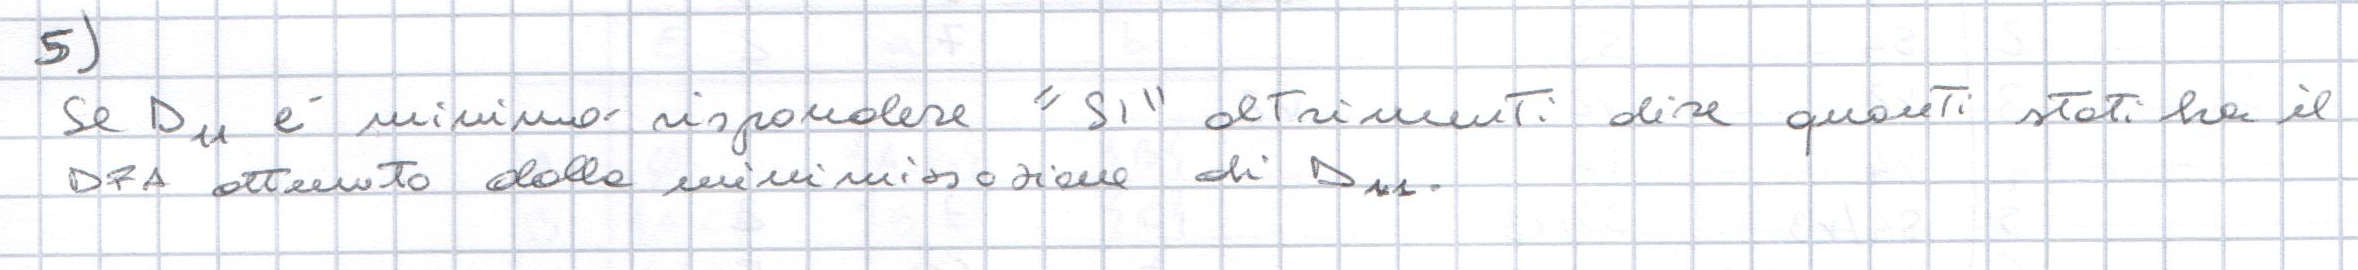
\includegraphics[scale=0.2]{Chapters/Img/05text.png}\\
\end{center} 

\subsection{Soluzione}

\begin{center}
    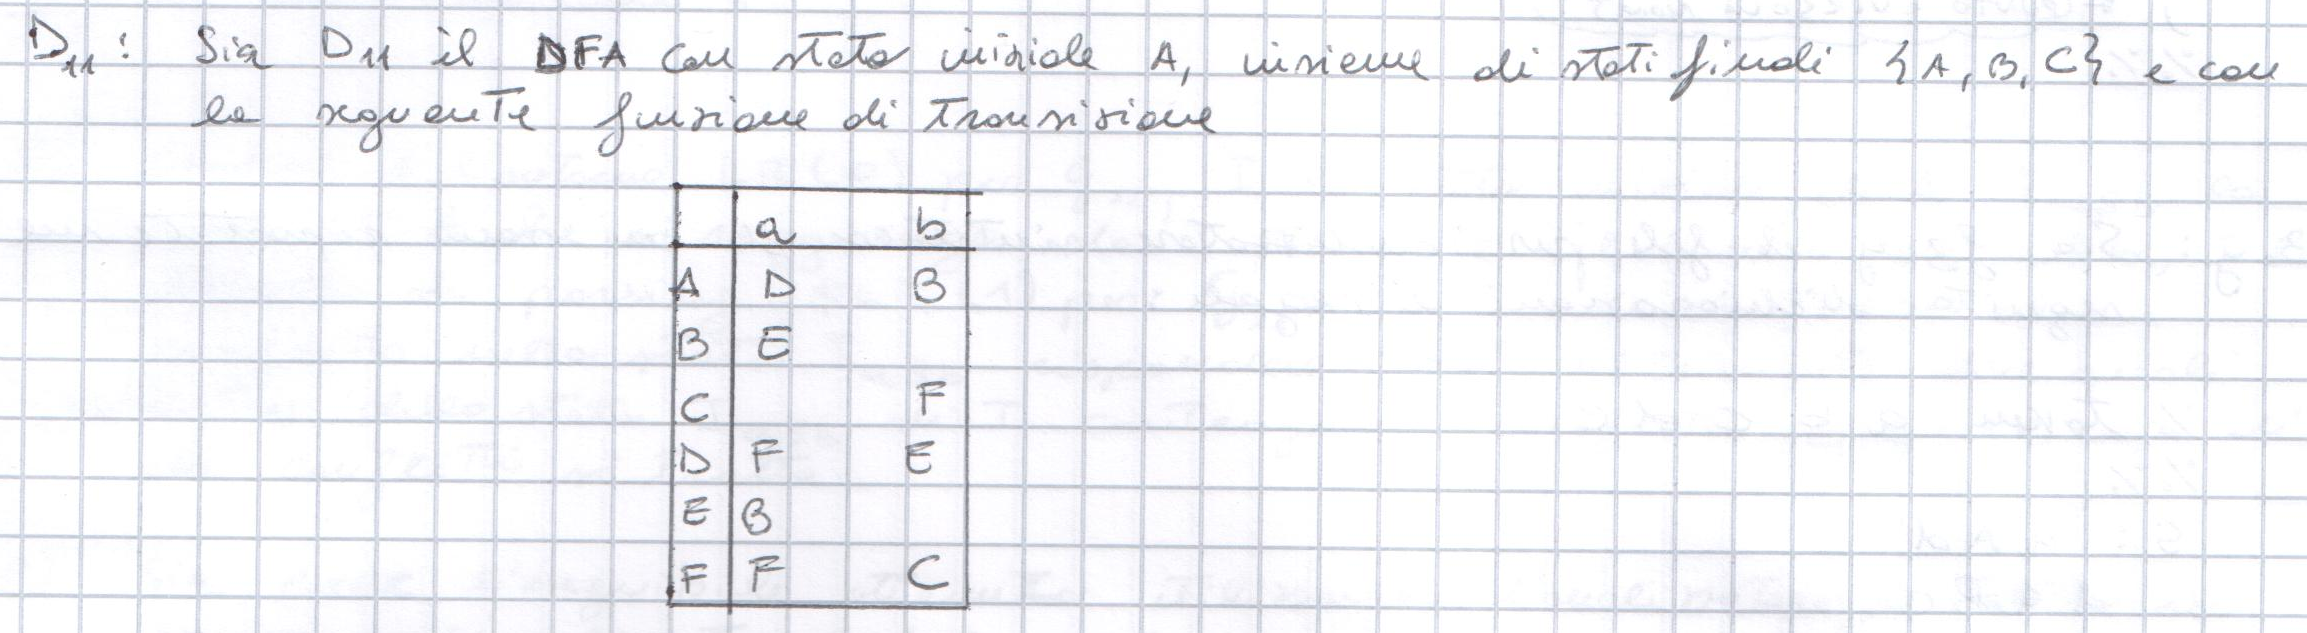
\includegraphics[scale=0.2]{Chapters/Img/d11.png}\\
    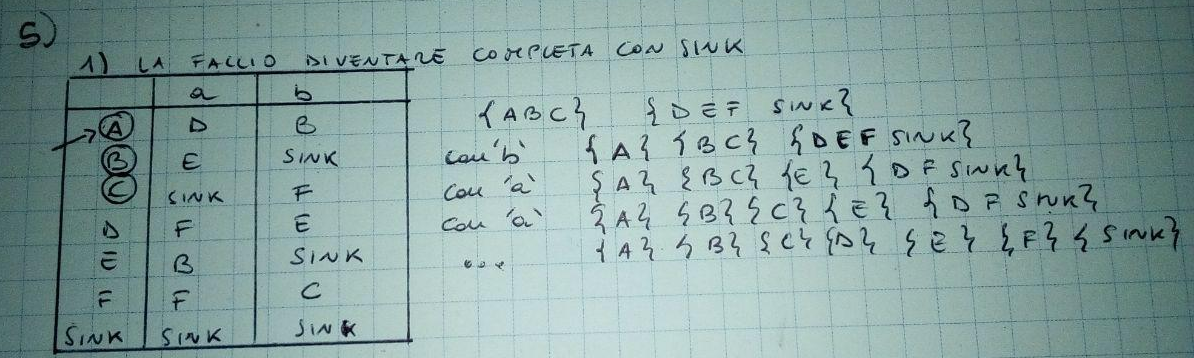
\includegraphics[scale=0.5]{Chapters/Img/05solution.png}\\
\end{center} 

\subsection{Risposta}
S\'i
\chapter{Esercizio 6}

\subsection{Testo}

\begin{center}
    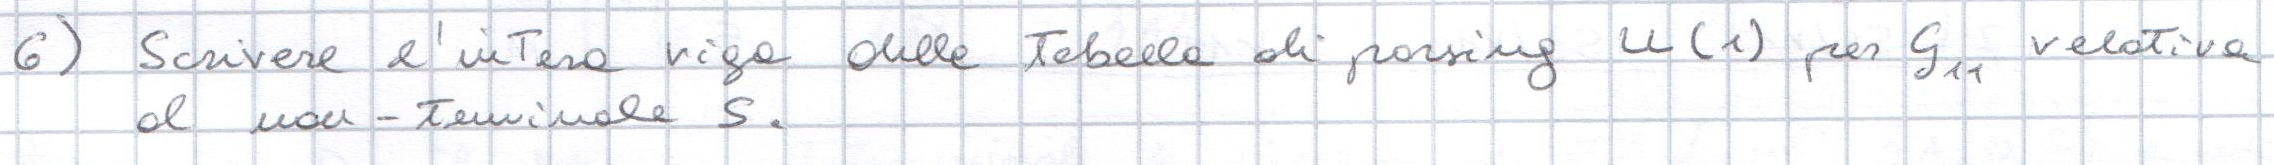
\includegraphics[scale=0.2]{Chapters/Img/06text.png}\\
\end{center} 

\subsection{Soluzione}



\subsection{Risposta}

\begin{tabular}{|c|cccc|}
    \hline
        &   a   &   b   &   c   &   $\$$    \\
    \hline
    S   &   $S \rightarrow aSbS $ & $S \rightarrow bSaS$ & $S \rightarrow cA$ & $S \rightarrow \varepsilon$ \\
        &   $S \rightarrow \varepsilon$ &  $S \rightarrow \varepsilon$ & & \\
    \hline
\end{tabular}
\chapter{Esercizio 7}

\subsection{Testo}

\begin{center}
    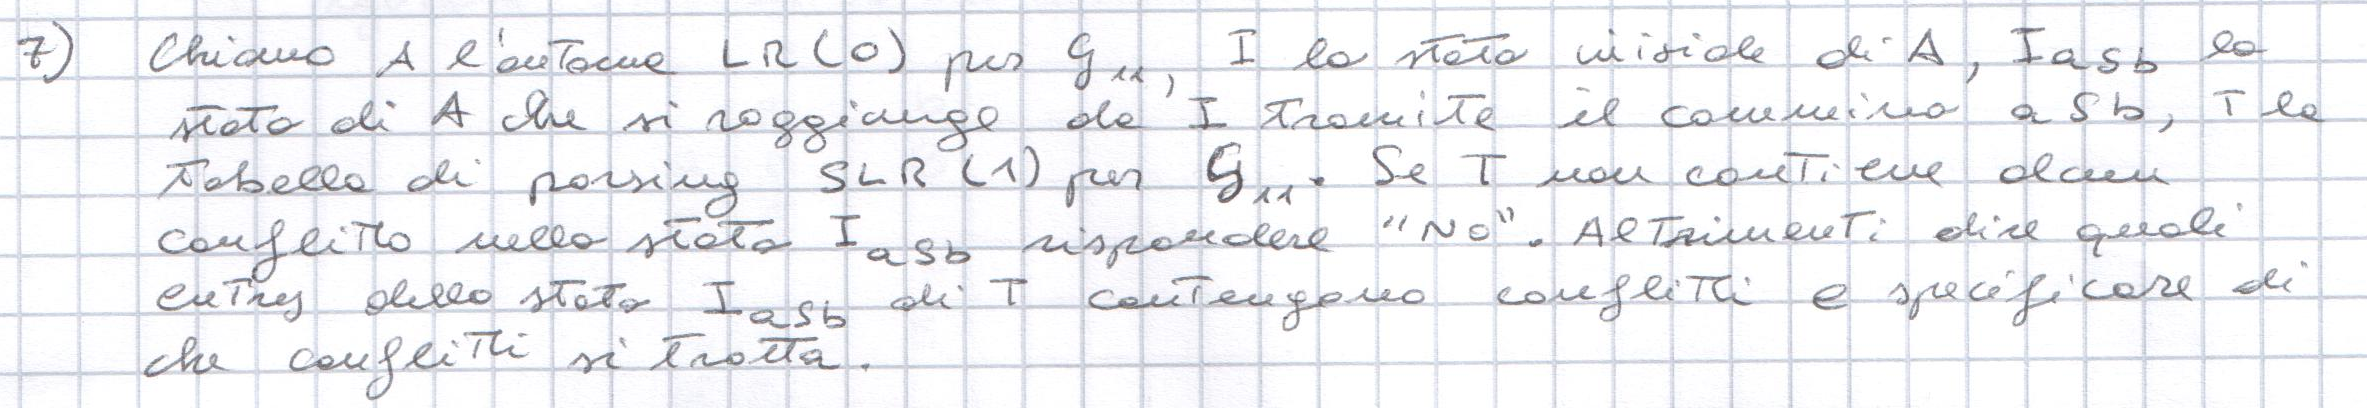
\includegraphics[scale=0.2]{Chapters/Img/07text.png}\\
    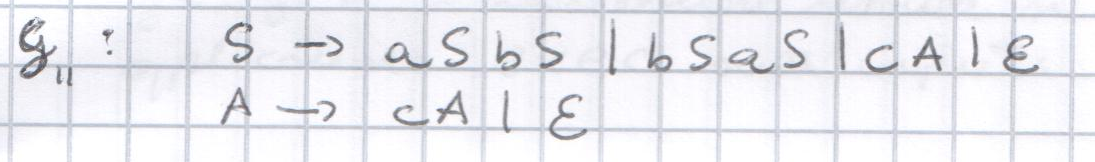
\includegraphics[scale=0.2]{Chapters/Img/g11.png}\\
\end{center} 

\subsection{Soluzione}

\begin{center}
    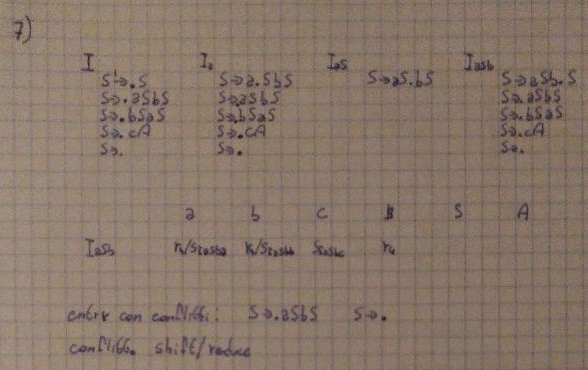
\includegraphics[scale=0.6]{Chapters/Img/07solution.png}\\
\end{center} 

%\subsection{Risposta}
\chapter{Esercizio 8}

\subsection{Testo}

\begin{center}
    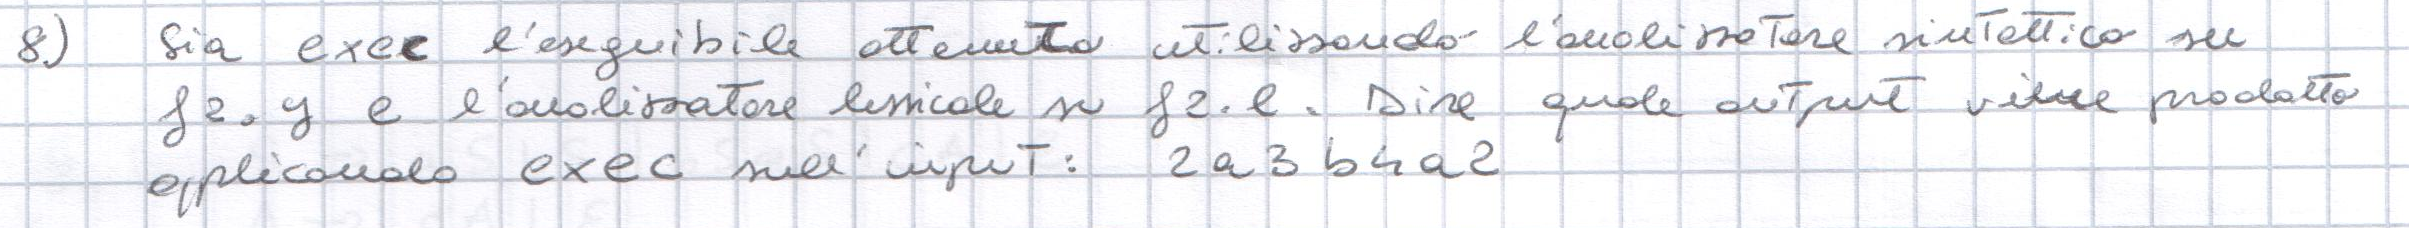
\includegraphics[scale=0.2]{Chapters/Img/08text.png}\\
\end{center} 

\subsection{Soluzione}
f2.y
\begin{lstlisting}
    %{
    #include <stdio.h>
    #include <stdlib.h>
    
    int yylex();
    int yyparse();
    void yyerror(char *s);

    %}

    %token a b num

    %%
    S: S E '\n' { printf("%d\n", $2); }
    | ;
    E: num { $$ = $1; }
    | E a E { $$ = $1 * $3; }
    | E b E { $$ = $1 + $3; } ;
    %%

    int main() {
    yyparse();
    return 0;
    }

    void yyerror(char *s) {
    printf("Error when reading: %s", s);
    }
\end{lstlisting}

f2.l
\begin{lstlisting}
    %option noyywrap

    %{
    #include "y.tab.h"
    #include <stdio.h>
    %}

    %%

    "a"   { return a; }
    "b"   { return b; }
    [0-9]+  { yylval = atoi(yytext); return num; }
    [-+\n]  return *yytext;
    [ \t]  ;
    .   yyerror("Invalid character");

    %%
\end{lstlisting}

\subsection{Risposta}
Input: 2a3b4a2
Output: 22

In pratica la scansione della stringa avviene da sinistra a 
destra ma essendo che Yacc usa tecniche bottom-up basate su 
tabelle LR mi ritorna una rightmost derivation pertanto matchano 
prima 4a2 poi 3b8 poi 2a11
\chapter{Esercizio 9}

\subsection{Testo}

\begin{center}
    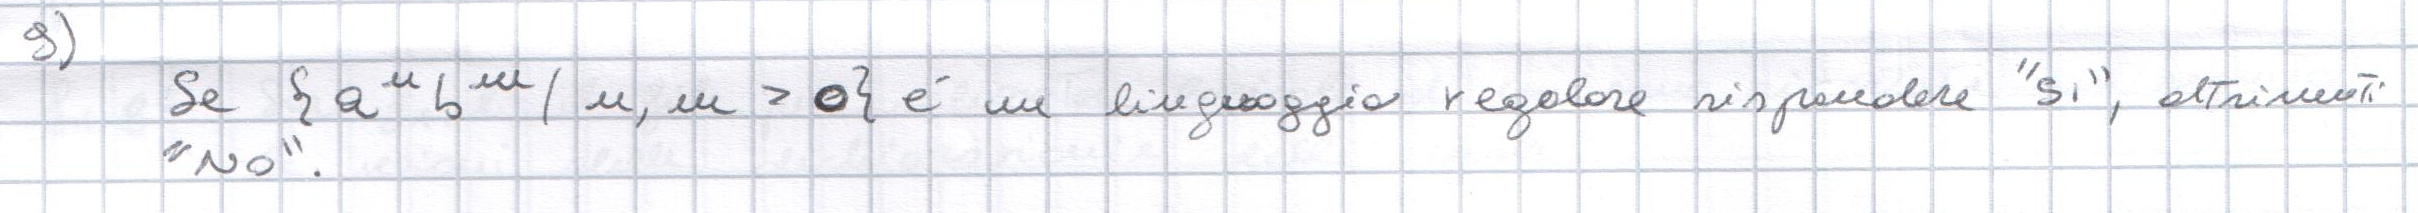
\includegraphics[scale=0.2]{Chapters/Img/09text.png}\\
\end{center} 

\subsection{Soluzione}
\'E regolare dato che la grammatica regolare G lo genera:\\
$S \rightarrow aS | aA $\\
$A \rightarrow bA | b $\\


\subsection{Risposta}
S\'i \'e regolare
\chapter{Esercizio 10}

\subsection{Testo}

\begin{center}
    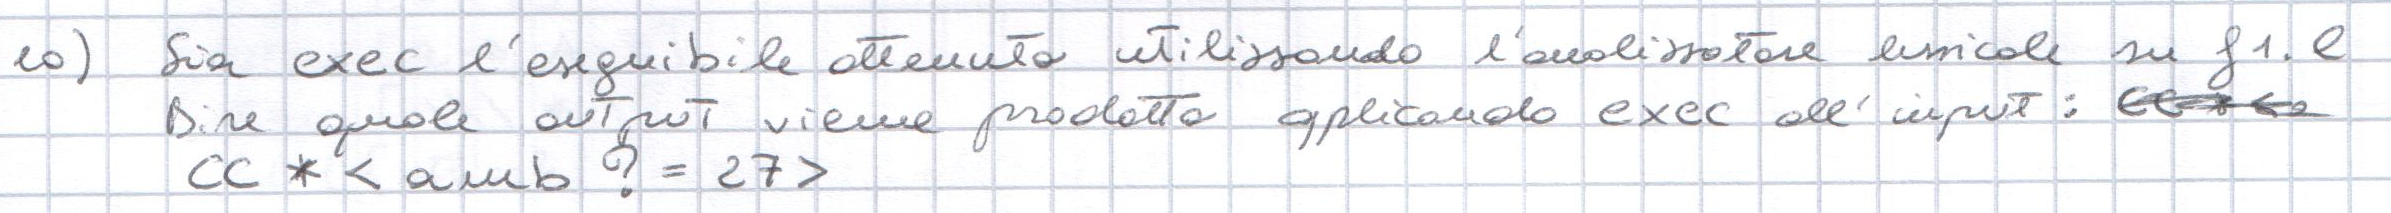
\includegraphics[scale=0.2]{Chapters/Img/10text.png}\\
\end{center} 

\subsection{Soluzione}
f1.l
\begin{lstlisting}
    %{
    
    %}

    digit [0-9]
    letters [a-z,A-Z]
    other [\\\*\?"<"]
    id ({other}|{digit}|{letters})+

    %%
    ({other})?({other})?({id})({digit})+({id})?   {printf("SI ");}
    {id}   {printf("FORSE ");}
    .   {printf("NO ");}

    %%
    int yywrap() {
    return 1;
    }

    int main() {
    yylex();
    }
\end{lstlisting}

\subsection{Risposta}
\begin{lstlisting}
    Input: CC*<amb?=27> 
    Output: FORSE NO SI NO
\end{lstlisting}
\chapter{Esercizio 11}

\subsection{Testo}

\begin{center}
    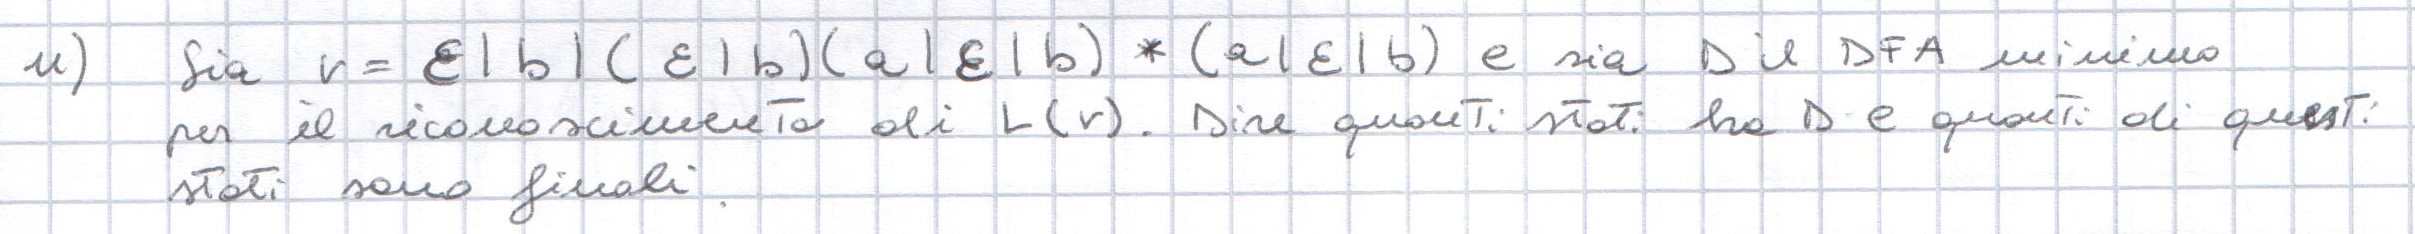
\includegraphics[scale=0.2]{Chapters/Img/11text.png}\\
\end{center} 

\subsection{Soluzione}

\subsection{Risposta}
4 stati finali
\chapter{Esercizio 12}

\subsection{Testo}

\begin{center}
    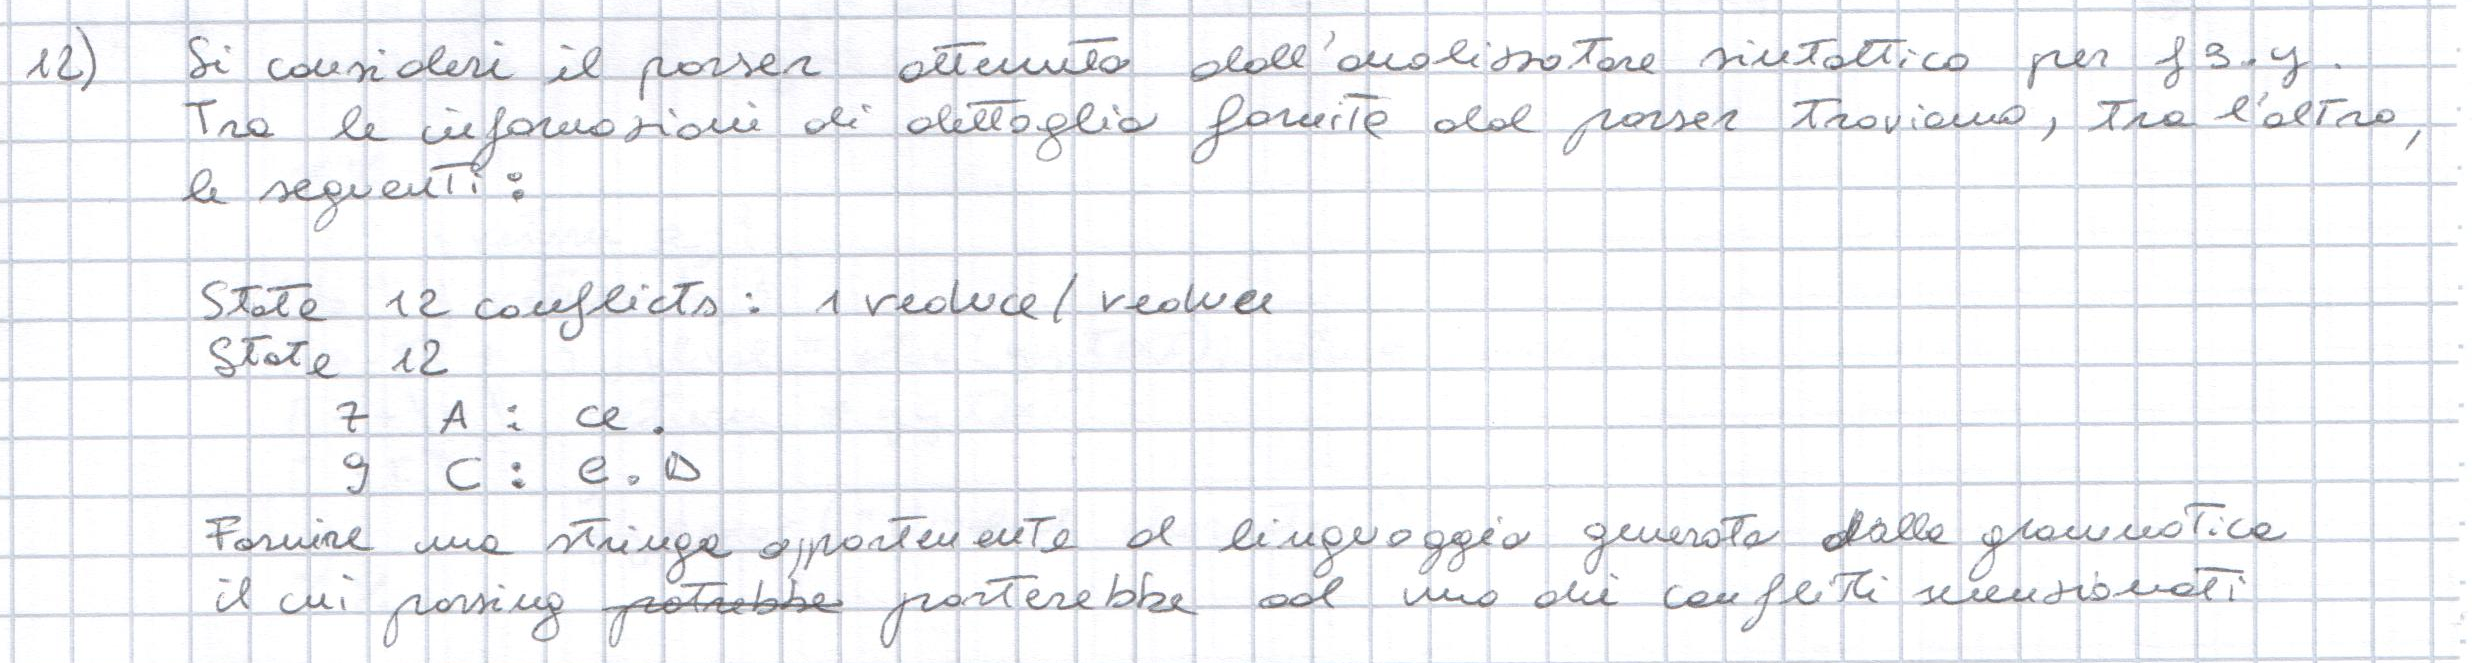
\includegraphics[scale=0.2]{Chapters/Img/12text.png}\\
\end{center} 

\subsection{Soluzione}
y3.y
\begin{lstlisting}
    %token a b c d e
    %%
    S:  aAd
        |baAe 
        |baBD 
        |cAd 
        |cBc
    ;
    A:  ce
    ;
    B:  cC
    ;
    C:  eD
    ;
    D:
    ;
    %%
\end{lstlisting}

\subsection{Risposta}
bacee
\chapter{Esercizio 13}

\subsection{Testo}

\begin{center}
    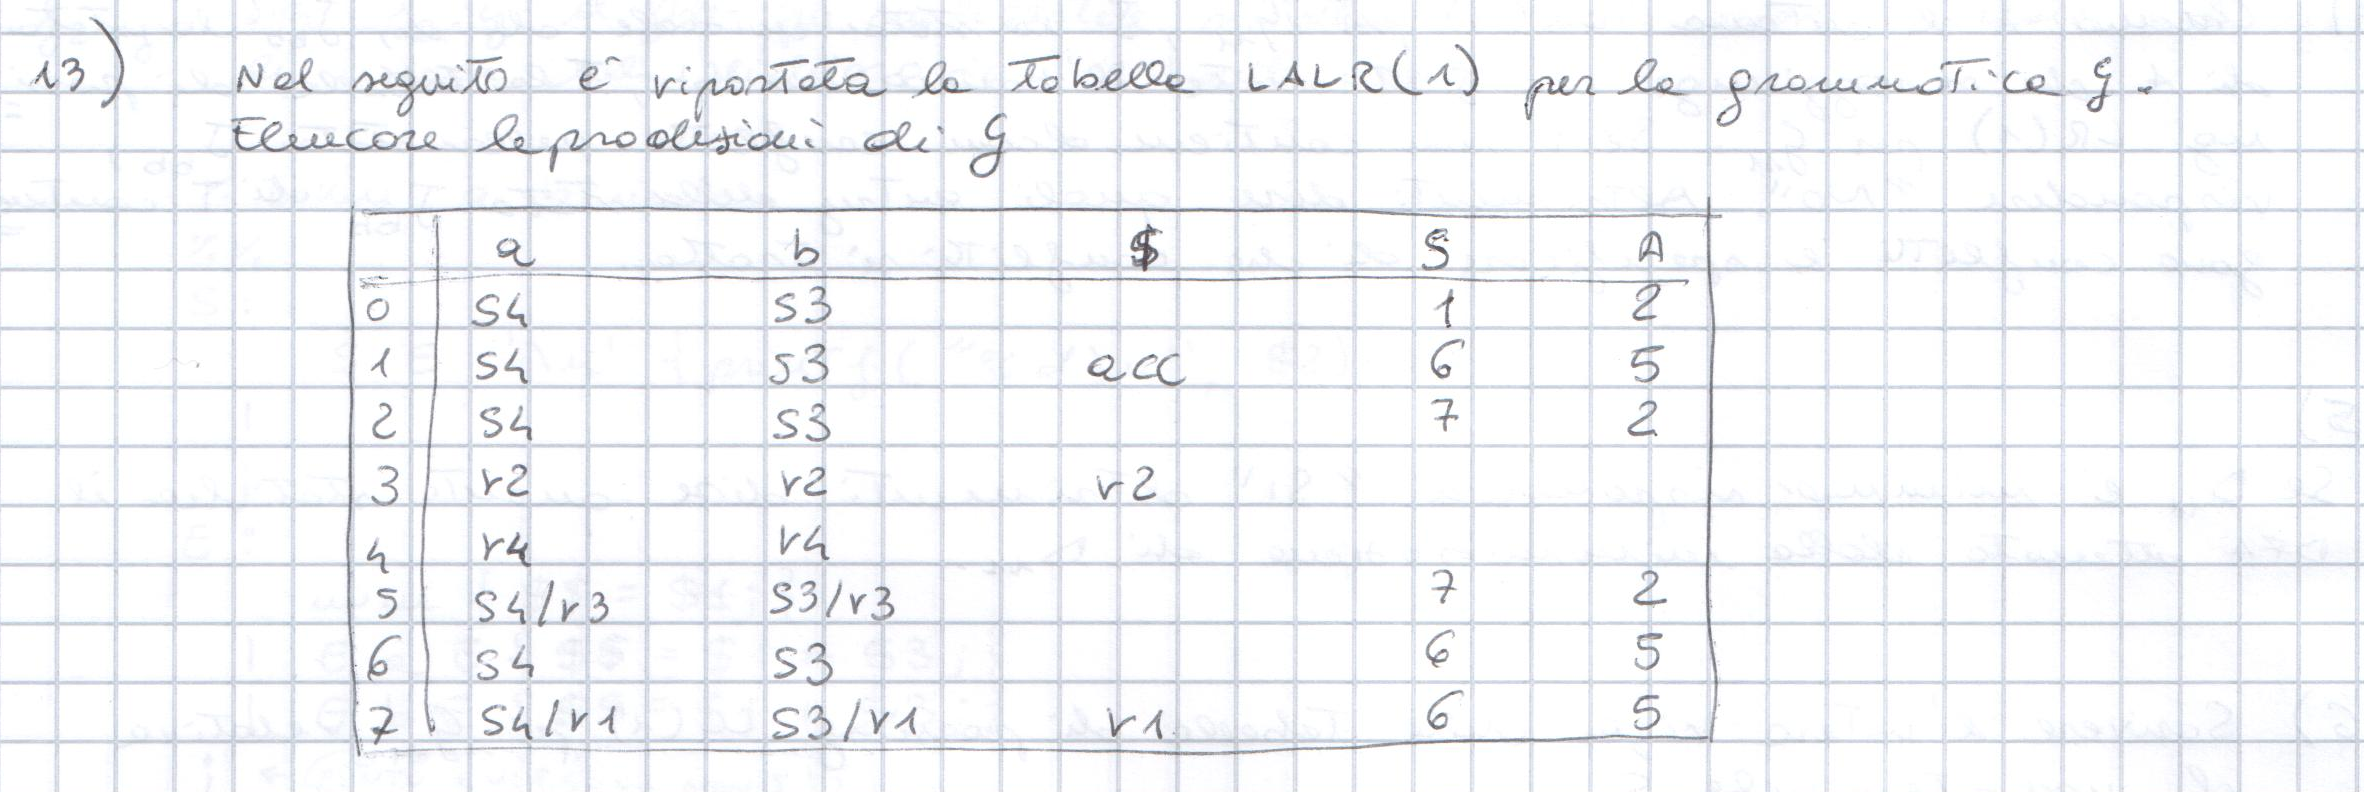
\includegraphics[scale=0.2]{Chapters/Img/13text.png}\\
\end{center} 

\subsection{Soluzione}

\subsection{Risposta}
\end{document}